%!TEX root = ../../../main.tex

\section{Abstract Model Checking and CEGAR}

\begin{frame}{Abstract Model Checking}
\begin{itemize}
  \itemsep1em
  
  \item For finite-state programs, symbolic reachibility analysis may take
  an large amount of time or memory to terminate
  
  \item Abstract model checking trades off precision of the analysis for
  efficiency
  
  \item Reachability analysis is performed on an abstract domain which
  captures some, but not necessarily all of the information about the system
  
  \item Abstract reachibility analysis is sound
  
  \item Model checking and static program analysis are both envolved in
  improving abstraction techniques \\
    \begin{itemize}
      \itemsep 0.3cm
      \item Model checking emphasizes precision
      \item Static program analysis emphasizes efficiency
    \end{itemize}   
\end{itemize}
\end{frame}

% ---------------------------------------------------------------------

\begin{frame}{Abstract Model Checking}

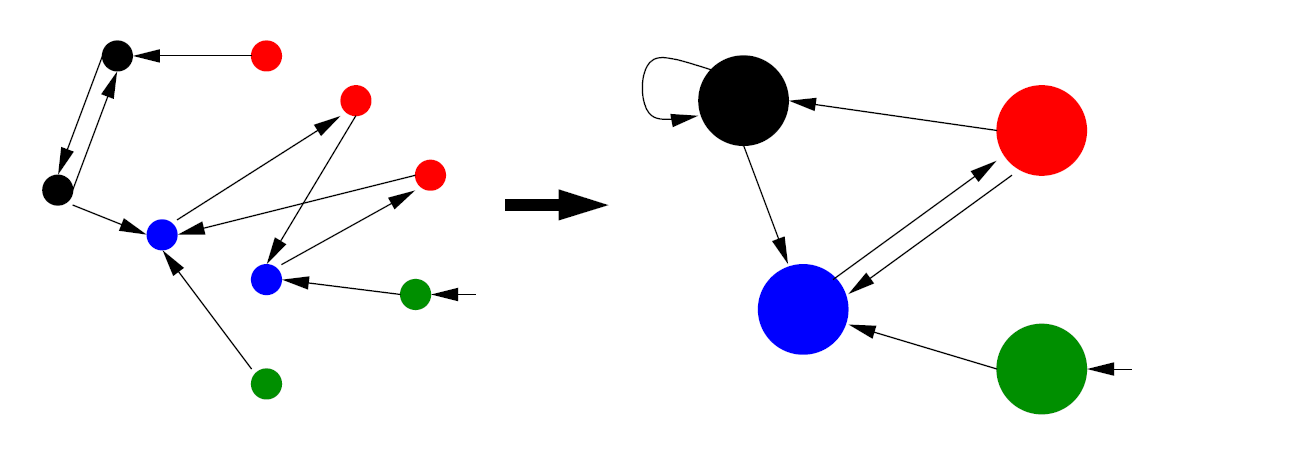
\includegraphics[width=\textwidth]{content/chapter_model_checking/software_model_checking/img/abstract.png}

\end{frame}

% ---------------------------------------------------------------------

\begin{frame}{Abstract Model Checking}
\begin{itemize}
  \itemsep1em
   
  \item Assume an abstract model $S_a$ of the concrete model $S_c$ such that
    $S_a \models \varphi \Rightarrow S_c \models \varphi$
  
  \item If a counterexample found in $S_a$, i.e. $S_a \models \neg \varphi$,
  then the abstract model has to be refined
  
  \item Refinement is repeated until the property is found to be true or a
  concrete a concrete counterexanple is found
  
  \item An abstract model $S_a$ is built using the \hl{Predicate abstraction}
  technique
  
  \item \hl{Counterexample-Guided Abstraction Refinement} (CEGAR)  
\end{itemize}
\end{frame}

% ---------------------------------------------------------------------

\begin{frame}{CEGAR}
\resizebox{1.05\textwidth}{!}{
  	\begin{tikzpicture}[>=stealth',shorten >=1pt,auto, node distance=3cm]
	 	\tikzstyle{rect} = [draw, rectangle, align=left,
	 	minimum width=2cm, minimum height=1cm]    
  			
  		\node[rect] (1) [] {Predicate \\ Abstraction};
  		\node[rect] (2) [right = of 1.east] {Model- \\ Checking};	
 		\node[rect] (3) [below of = 1] {Predicate \\ Refinement};
 		\node[rect] (4) [below of = 2] {Spurious ?};
 		
 		\node[node distance=1.8cm] (01) [left = of 1.west] {};
 		\node[node distance=1.8cm] (02) [right = of 2.east] {};
 		\node[node distance=1.8cm] (04) [right = of 4.east] {};
 		
 		\node[rectangle, draw, 
 		minimum width=7.6cm, minimum height=4.5cm, fit= (1) (2) (3) (4)] {};
 		
 		\path[->] 	(1)	edge node {Boolean program} (2)
 					(1)	edge[below] node {$\varphi$} (2)
 					
 					(2)	edge[left] node {Counter-example (CE)} (4)
 					(4)	edge[below] node {Spurious !} (3)
 					
 					(3)	edge[below] node {} (1)
 					
 					(01) edge node {Prog $P$} (1)
 					(01) edge[below] node {Spec $\varphi$} (1)
 					
 					(2) edge node {$\varphi$} (02)
 					
 					(4) edge node {$\neg \varphi$} (04)
 					(4) edge[below] node {CE} (04)					
 		; 					 				
	\end{tikzpicture}
  
}
\end{frame}

% ---------------------------------------------------------------------

\begin{frame}{CEGAR and Lazy Abstraction}
\resizebox{1.05\textwidth}{!}{
    \begin{tikzpicture}[>=stealth',shorten >=1pt,auto, node distance=3cm]
    \tikzstyle{rect} = [draw, rectangle, align=left,
    minimum width=2cm, minimum height=1cm]    
        
      \node[rect] (1) [] {\hl{Cartesian} \\ \hl{Abstraction}};
      \node[rect] (2) [right = of 1.east] {Explicit MC};  
    \node[rect] (3) [below of = 1] {\hl{Predicate} \\ \hl{Refinement}};
    \node[rect] (4) [below of = 2] {Spurious ?};
    
    \node[node distance=1.8cm] (01) [left = of 1.west] {};
    \node[node distance=1.8cm] (02) [right = of 2.east] {};
    \node[node distance=1.8cm] (04) [right = of 4.east] {};
    
    \node[rectangle, draw, 
    minimum width=7.6cm, minimum height=4.5cm, fit= (1) (2) (3) (4)] {};
    
    \path[->]   (1) edge node {$\hl{ART}$} (2)
          (2) edge[below] node {\hl{on-the-fly}} (1)
          
          (2) edge[left] node {Counter-example (CE)} (4)
          (4) edge[below] node {Spurious !} (3)
          
          (3) edge[below] node {} (1)
          
          (01) edge node {$\hl{CFA_\varphi}$} (1)        
          
          (2) edge node {$\varphi$} (02)
          
          (4) edge node {$\neg \varphi$} (04)
          (4) edge[below] node {CE} (04)          
    ;
          
          
  \end{tikzpicture}  
}
\end{frame}

% ---------------------------------------------------------------------

\begin{frame}{Control-Flow Automata (CFA)}
\begin{itemize}
  \itemsep1em 
  \item We consider simple imperative programs where all operations are either
  assignements or assume operations
  \item We represent a program by a \hl{control-flow automaton} $A =
  (L, G)$ where
    \begin{itemize}
      \itemsep 0.1cm 
      \item $L$ - is a set of program locations
      \item $G \subseteq L \times Ops \times L$ - is a set of control flow edges
  \end{itemize}
  \item A \hl{program} $P = (A, l_0, l_E)$ consist of a CFA $A = (L, G)$ and
  propgram locations $l_0, l_E \in L$ s.t.
    \begin{itemize}
      \itemsep 0.1cm
      \item $l_0$ - models an initial program location, and
      \item $l_E$ - models the error location
  \end{itemize}
  \item MC Problem: does the location $l_E$ is reachable from the location $l_0$
  in $P$
\end{itemize}
\end{frame}

% ---------------------------------------------------------------------

\begin{frame}[fragile]{Control-Flow Automata (CFA)}
\begin{columns}
  \begin{column}{0.6\textwidth}    
    \begin{overprint}
      \onslide<1-2>
        
\begin{figure}[htbp]
  \begin{center}
	\begin{tikzpicture}[>=stealth',shorten >=1pt,auto,node distance=1.2cm]
	 	
	 	 \onslide<1->{   	 	    
  			\node[loc] (1) []  	{$0$};		
  			\node[loc] (2) [below of = 1] 	{$1$};
 			  \node[loc] (3) [right of = 2, node distance=2cm]	{$2$};		
 			
 			  \node[loc] (4) [below of = 2]	{$3$};
 			  \node[loc] (5) [below of = 4]	{$4$};

        \path[trans]
          (1) edge [left] node {$i := 0$} (2)       
          (2) edge [left] node {$i > 5$} (4)

          (2) edge [above, bend left = 20] node {$i \leq 5$} (3)
          (3) edge [below, bend left = 20] node {$i := i + 1$} (2)          
          ;    		
 		} 		
 		
    \onslide<1>{
        \path[trans]
          (4) edge [left] node {$result := i$} (5)
        ;
    }

 		\onslide<2->{ 		
 			\node[loc] (6) [below of = 5]	{$5$};
 			\node[loc, fill=red!50] (7) [right of = 5]	{$\mathcal{E}$}; 		
 		}
 		 		
 		\onslide<2->{
 			\path[trans] 				
 				(5) edge [left] node {$result := i$} (6)
 			
 				(4) edge [left] node {$i = 6$} (5)
 				(4) edge [right] node {$i \neq 6$} (7)	
 			;		
 		}
 		
 		
	\end{tikzpicture}
  \end{center}
\end{figure}
    \end{overprint}
  \end{column}
  \begin{column}{0.4\textwidth}
    \begin{overprint}
    \onslide<1->
      \begin{example}   
        \begin{lstlisting}[escapechar=\%]
  i := 0
  while(i <= 5) {
    i := i + 1
  }
  result := i
        \end{lstlisting}
      \end{example}
    \onslide<2->{ 
      \hl{Assertion}: \\ $i = 6$ after the loop
    }
    \end{overprint} 
  \end{column}
\end{columns}
\end{frame}

% ---------------------------------------------------------------------

\begin{frame}{Control-Flow Automata (CFA)}
\begin{itemize}
  \itemsep1em 
  \item A \hl{concrete data state} of a program is a variable assignment $c:
  X \rightarrow D$ where $D$ is some non-empty domain
  
  \item We represent sets of concrete data states symbolically using first-order
  formulas \\
  \begin{itemize}
    \item an FO-formula $\varphi$ represents the set $S$ of all data states $c$
    that imply $\varphi$, i.e. $S = \{ c \ | \ c \models \varphi \}$
  \end{itemize}
  \item A \hl{concrete state} of a program is a pair $(l, c) \in L \times S$
  
  \item The \hl{concrete semantics} of an operation $op \in Ops$ is defined by
  the \hl{strongest postcondition} operator $SP_{op}$ as \\
    \begin{itemize}
      \itemsep 0.2cm 
      \item $SP_{x := e}(\varphi) = \exists x': \varphi_{[x \mapsto x' ]} \wedge
      (x = e_{[x \mapsto x']})$
      \item $SP_{p}(\varphi) = \varphi \wedge p$ where $p$ is a conditional, e.g. $i \leq 5$
    \end{itemize}
\end{itemize}

\end{frame}

% ---------------------------------------------------------------------

\begin{frame}{Cartesian Predicate Abstraction}
\begin{itemize}
  \itemsep1em 
  \item The \hl{predicate abstraction} domain is parameterized by a fixed
  finite set of first-order formulas $\pi$ with free variables from the
  program variables
  
  \item A \hl{cartesian predicate abstraction} $\varphi^\pi$ of a
  formula $\varphi$ is the strongest conjunction of predicates from
  $\pi$ that is entailed by $\varphi$:
    \begin{align*}
      \varphi^\pi := \bigwedge \{ p \in \pi \ | \ \varphi \Rightarrow p \}
    \end{align*}
  
  \item The abstract strongest postoperator $SP^\pi$ for the predicate
  abstraction $\pi$ is defined as:
    \begin{align*}
      SP_{op}^{\pi}(\varphi^\pi) =
      (SP_{op}(\varphi^\pi))^{\pi}
    \end{align*} 
\end{itemize}

\end{frame}

% ---------------------------------------------------------------------

\begin{frame}{Abstract Reachibility Tree (ART)}
\begin{itemize}
  \itemsep1em 
  
  \item An ART is a tree whose nodes are labeled with program locations and
  abstract states, i.e. $(l, \varphi^\pi)$
  
  \item A node $n = (l, \varphi)$ is \hl{covered} if there exists another
  node $n' = (l, \varphi')$ s.t. $\varphi' \models \varphi$
  
  \item An ART is \hl{complete} if every leaf node is covered
  
  \item Given a program $P = (A, l_0, l_E)$ and a set of predicates $\pi$,
  starting from the abstract state $(l_0, \{ \top \})$ we construct an
  \hl{abstract reachibility tree} (ART) using the abstract postoperator $SP^\pi$   
  
  \item If a complete ART is constructed and does not contain any error node
  $(l_E, \varphi)$, the program is considered correct
  
\end{itemize}
\end{frame}

% ---------------------------------------------------------------------

\begin{frame}{Abstract Reachibility Tree (ART)}
$\pi_0 = \{ i = 0\}$
\begin{columns}
  \begin{column}{0.5\textwidth}   
    
\begin{figure}[htbp]
  \begin{center}
	\begin{tikzpicture}[>=stealth',shorten >=1pt,auto,node distance=1.2cm]
		
		 	\node[loc] (1) []  	{$0$};		
  			\node[loc] (2) [below of = 1] 	{$1$};
 			\node[loc] (3) [right of = 2, node distance=2cm]	{$2$};		
 			
 			\node[loc] (4) [below of = 2]	{$3$};
 			\node[loc] (5) [below of = 4]	{$4$};
 			
 			\node[loc] (6) [below of = 5]	{$5$};
 			\node[loc, fill=red!50] (7) [right of = 5]	{$\mathcal{E}$};	 	
	 	 
	
 			\path[trans]  			
 				(1) edge [left] node {$i := 0$} (2)				
				(2) edge [left] node {$i > 5$} (4)									 						
 			;
 			

 			\path[trans]
 				(2) edge [above, bend left = 20] node {$i \leq 5$} (3)
 				(3) edge [below, bend left = 20] node {$i := i + 1$} (2)
 				
 				(5) edge [left] node {$result := i$} (6)
 			
 				(4) edge [left] node {$i = 6$} (5)
 				(4) edge [right] node {$i \neq 6$} (7)	
 			;				
 		
 		
	\end{tikzpicture}
  \end{center}
\end{figure}
  \end{column}  
  \begin{column}{0.5\textwidth}
    
\begin{figure}[htbp]
  \begin{center}
	\begin{tikzpicture}[>=stealth',shorten >=1pt,auto,node distance=1.2cm]
		
		 	\node[artloc={$\{ \}$}] (0) []  	{$0$};		
  			\node[artloc={$\{ i = 0 \}$}] (1) [below of = 0] 	{$1$};
 			\node[artloc={$\{ i = 0 \}$}] (2) [below of = 1]	{$2$};		
 			
 			\node[artloc={$\{ \}$}] (11) [below of = 2] 	{$1$};
 			
 			\node[artloc={$\{ \}$}] (3) [below of = 11]	{$3$};
 			
 			\node[artloc={$\{ \}$}, fill=red!50] (7) [below of = 3]	{$\mathcal{E}$};	 	
	 	 
	
 			\path[trans]  			
 				(0) edge [left] node {$i := 0$} (1)				
				(1) edge [left] node {$i \leq 5$} (2)
				(2) edge [left] node {$i := i + 1$} (11)				 						
 				(11) edge [left] node {$i > 5$} (3)
 				(3) edge [left] node {$i \neq 6$} (7)					
 			;				
 		
 		
	\end{tikzpicture}
  \end{center}
\end{figure}
  \end{column}
  
\end{columns}
\end{frame}

% ---------------------------------------------------------------------

\begin{frame}{Abstraction refinement}
\resizebox{1.05\textwidth}{!}{
  \begin{tikzpicture}[scale=0.75]

\tikzset{trans/.style={%
  ->,
  onslide=<2->{opacity=.1}
}}

\tikzset{atrans/.style={%
  ->,
  onslide=<3>{opacity=.1}
}}


\tikzset{cetrans/.style={%
  ->, 
  onslide=<3>{opacity=1}
}}


\tikzset{loc/.style={%
  state,
    minimum width=0.2cm,
    minimum height=0.2cm,
    onslide=<2->{opacity=.1}      
}}


\tikzset{celoc/.style={%
  state,
    minimum width=0.2cm,
    minimum height=0.2cm,
  onslide=<2>{opacity=.1}      
}}


\onslide<2->{
\fill[green!30]  plot[smooth cycle, tension=.7] coordinates 
  {(-14.5,2.5) (-13,1) (-11.5,1.5) (-13.5,3)};

\fill[pink]  plot[smooth cycle, tension=.7] coordinates 
  {(-4.5,6.5) (-1,5) (-1,6) (-4,7)};
 
\fill[blue!30]  plot[smooth cycle, tension=.7] coordinates {
  (-10.5,3) (-9.5,1) (-5,0.5) (-5,3) (-7,3.5)};
}


\onslide<2-3>{
\fill[yellow!50]  plot[smooth cycle,tension=.7] coordinates 
  {(-13,5) (-11.5,3.5) (-7.5,4.5) (-8.5,6.5) (-11.5,6)};

\fill[gray!50]  plot[smooth cycle, tension=.7] coordinates 
  {(-6.5,6) (-5.5,4) (-4,2.5) (-2.5,2) (-2,3.5) (-4,5) (-5,6.5)};
}

% Refined
\onslide<4->{
\fill[gray!50]  plot[smooth cycle, tension=.7] coordinates 
{(-5.5,5) (-5.5,4) (-4,2.5)(-2.5,2) (-2,3.5) (-3.5,4.5) (-4.5,5)};

\fill[yellow!50] plot[smooth cycle, tension=.7] coordinates 
{(-12.5,4) (-11.5,3.5) (-8.5,4) (-8.5,5) (-11.5,4.5)};

\fill[cyan!50]  plot[smooth cycle, tension=.7] coordinates 
{(-12,6) (-12,5) (-5,5.5) (-5,6.5) (-8.5,6.5)};
}



\node[loc, fill=green] (v13) at (-13.5,2.5) {};
\node[loc, fill=green] (v14) at (-12.5,1.5) {};
\node[loc, fill=red] (v9) at (-1.5,5.5) {};
\node[loc] (v6) at (-4.5,4) {};
\node[loc] (v11) at (-8.5,1.5) {};
\node[loc] (v12) at (-11.5,4) {};

\node[loc] (v3) at (-8.5,4.5) {};

\node[loc] (v10) at (-5.5,1.5) {};
\node[loc] (v7) at (-2.5,2.5) {};
\node[loc] (v8) at (-7,3) {};
\node[loc] (v15) at (-10,2.5) {};

% Counter-example
\node[celoc] (v1) at ((-11.5,5.5) {};
\node[celoc] (v2) at (-9,6) {};
\node[celoc] (v4) at (-5.5,6) {};
\node[celoc, fill=red] (v5) at (-3.5,6.5) {};

\draw[trans, cetrans]  (v1) edge (v2);


% Abstract transitions
% (yellow -> gray)
\draw[atrans, cetrans, onslide=<4->{opacity=.1}]  (v2) edge (v4); 
% (gray -> red)
\draw[atrans, cetrans]  (v4) edge (v5);
% (blue -> gray)
\draw[atrans]  (v10) edge (v7);
% (green -> yellow)
\draw[atrans]  (v13) edge (v12);
% (green -> blue)
\draw[atrans]  (v14) edge (v15);
% (yellow -> blue)
\draw[atrans]  (v3) edge (v8);


\draw[trans]  (v4) edge (v6);
\draw[trans]  (v6) edge (v7);
\draw[trans]  (v8) edge (v10);
\draw[trans]  (v11) edge (v10);
\draw[trans]  (v12) edge (v3);
\draw[trans]  (v15) edge (v8);
\draw[trans]  (v15) edge (v11);

%\draw[->]  (v12) edge (v1);

\end{tikzpicture}
}
\end{frame}

% ---------------------------------------------------------------------

\begin{frame}{Abstraction refinement}
\begin{itemize}
  \itemsep 1em 
  \item If during the construction of an ART we hit an error node, then we have
  to check whether the discovered path from the initial node $l_0$ to the error
  node $l_E$ exists in the concrete system
  
  \item The \hl{concrete semantics} for a program path 
  $\sigma = \langle (op_1, l_1), \ldots, (op_n, l_n) \rangle$, is defined as:
    \begin{align*}
      SP_\sigma(\varphi) = SP_{op_n}(\ldots SP_{op_1}(\varphi))
    \end{align*}
  
  \item A program path $\sigma$ is \hl{feasible} if $SP_\sigma(\top)$ is
  satisfiable, otherwise it is \hl{infeasible}
\end{itemize}
\end{frame}

% ---------------------------------------------------------------------

\begin{frame}{Abstraction refinement}
\begin{itemize}
  \itemsep 1em   
  \item If a discovered path is infeasible we have to refine the current
  abstraction, i.e. add new predicates to $\pi$
  
  \item In order to guarantee the termination of the algorithm the following 
  has to hold for the \underline{refined} set of predicates $\pi'$:
  \begin{align*}
      SP_{op_n}^{\pi'}(\ldots SP_{op_1}^{\pi'}(\top)) \models \bot
    \end{align*}
    
\end{itemize}
\end{frame}

% ---------------------------------------------------------------------

\begin{frame}{Abstraction refinement}
\begin{itemize}
  \itemsep 1em  
  \item We try to extract new predicates from the counterexample s.t.
    \begin{itemize}
      \itemsep 0.1cm
      \item the same counterxample will no be discovered in next interations
      \item predicates should be as precise as possible
      \item as few predicates as possible*
    \end{itemize}  
  \item There are two main techniques
    \begin{itemize}
      \itemsep 0.1cm
      \item Interpolants
      \item Weakest Preconditions / Strongest Postconditions
    \end{itemize}  
  \item Iterpolantion is the most widely used technique in all state of the art
  software model-checking tools (BLAST, CPAchecker)
    \begin{itemize}
      \itemsep 0.1cm
      \item mostly used for problems encoded over LRA theory
      \item lose of precision for the BV theory
      \item for the McCarthy's theory of arrays inapplicable princpially
    \end{itemize}        
\end{itemize}
\end{frame}

% ---------------------------------------------------------------------

\begin{frame}{Abstraction refinement}
\begin{itemize}
  \itemsep 0.3cm 
  \item Given a spurious counterexample $\sigma = \langle (op_1, l_1), \ldots,
  (op_n, l_n) \rangle$
  
  \item We define the refined set of predicates $\pi'$ as
  \begin{align*}
  \pi' = \pi \cup \bigcup_{i \in 1..n} \neg WP_{op_i}(\top) 
  \end{align*}  
  where
  \begin{align*}
  WP_{op_i}(\varphi) = WP(op_i, WP(op_{i + 1}, \ldots WP(op_n, \varphi))) 
  \end{align*}
  \item The weakest precondition operator is defined as:
      \begin{itemize}
      \itemsep 0.2cm 
      \item $WP_{x := e}(\varphi) = \varphi_{[x \mapsto e ]}$
      \item $WP_{p}(\varphi) = \varphi \wedge p$ where $p$ is a conditional, e.g. $i \leq 5$
    \end{itemize}    
\end{itemize}
\end{frame}

% ---------------------------------------------------------------------

\begin{frame}{Example 1}


\begin{figure}[htbp]
	\begin{tikzpicture}[>=stealth',shorten >=1pt,auto,node distance=2cm]
	 	
	 	\node (0) {ART$_0$: };
	 	
	 	\node[artloc={$\{ \}$}, node distance = 1cm] (1) 
	 		[right of = 0]	{$1$};
	 				
  		\node[artloc={$\{ \}$}] (2) 
  			[right of = 1] 	{$2$};	
 		
 		\node[artloc={$\{ \}$}] (4) 
 			[right of = 2]	{$4$};
 		
 		\node[artloc={$\{ \}$}] (6) 
 			[right of = 4]	{$\mathcal{E}$};
 				 
		\path[trans]  
 			
 			(1) edge node [below] {$i := 0$} 	(2)
			(2) edge node [below] {$i > 5$}		(4)	
			(4) edge node [below] {$i \neq 6$}	(6)		 									
 			;
 					
	\end{tikzpicture}
\end{figure}
\begin{itemize}
%   \item UNSAT-Core: \quad 
%   $i_1 = 0 \ \wedge \ i_2 = i_1 \ \wedge \ i_2 > 5$
  
  \item Compute WP for the following program: 
  \begin{gather*} 
  \onslide<5->{{\color{red} \{0 > 5 \wedge 0 \neq 6\}} } \\
  i := 0 \\
  \onslide<4->{ {\color{blue} \{ i > 5 \wedge i \neq 6 \} } }
  \\
  i > 5 \\
  \onslide<3->{ {\color{blue} \{ i \neq 6 \}} }
  \\
  i \neq 6 \\
  \onslide<2->{ {\color{blue} \{ \top \}} }
  \end{gather*}
  
  \item<5-> Extracted predicates: $\{ i = 6; \ i \leq 5 \vee i = 6 \}$
\end{itemize}
\end{frame}


% ---------------------------------------------------------------------

\begin{frame}{Example 2}
\begin{figure}
\resizebox{\textwidth}{!}{
  

\begin{tikzpicture}[>=stealth',shorten >=1pt,auto,node distance=1.7cm]
	 	
	 	\node (0) {ART$_1$: };
	 	
	 	\node[artloc={$\{ \}$}, node distance = 1cm] (1) 	
	 		[right of = 0]	{$1$};		
  		
  		\node[artloc={$\{i \leq 6\}$}] (2) 	
  			[right of = 1] 	{$2$};
  		
  		\node[artloc={$\{i \leq 6\}$}] (3) 	
  			[right of = 2] 	{$3$};
  		
  		\node[artloc={$\{\}$}] (22) 
  			[right of = 3, node distance = 2cm] 	{$2$};
 		
 		\node[artloc={$\{\}$}] (4) 
 			[right of = 22]	{$4$};
 		
 		\node[artloc={$\{\}$}] (6) 
 			[right of = 4]	{$\mathcal{E}$};
 				 
		\path[trans]  
 			
 			(1) edge node [below] {$i := 0$} 	(2)
 			(2) edge node [below] {$i \leq 5$}	(3)
			(3) edge node [below] {$i := i + 1$} (22)	
			(22) edge node [below] {$i > 5$}	(4)
			(4) edge node [below] {$i \neq 6$}	(6)	
 			;
 					
\end{tikzpicture}

}
\end{figure}

\begin{itemize}  
  \item Compute WP for the following program (short form):    
  \begin{gather*}
  \onslide<5->{{\color{red} \{ 0 + 1 > 5\}} } \\
  i := 0 \\
  \onslide<4->{{\color{blue} \{i + 1 > 5\}} } \\
  i := i + 1 \\
  \onslide<3->{ {\color{blue} \{ i > 5 \} } }
  \\
  i > 5 \\
  \onslide<2->{ {\color{blue} \{ \top \}} }
  \\
  \end{gather*} 
  \item<6-> Extracted predicates: $\{ i \leq 5; i \leq 4 \}$
  
\end{itemize}
\end{frame}
